We identified the potential sharing candidates (SEs) from the input queries, it is the goal of this phase to build the covering subexpressions (CEs) that are the ``covering" omputations. Given the sets of SEs, the optimizer first tries to eliminate obviously bad candidates for sharing with the help from the cost estimation. Then for each set of SEs, we construct a single CE to produce all common sharing tuples for the consumers (all SEs in that set). Some CEs might become \emph{cache plans} after the cost-based optimization in phase 3. 

In this paper, we define the \emph{cache plan} as the materialization for our idea. A \emph{cache plan} is a CE defining the result of a materialized view. In other words, cache plans can be seen as temporary views in RDBMSes and to be materialized in RAM. In our work, \emph{cache plans} (selected CEs) will be executed only once and the result is materialized in RAM so that it could be reused multiple times to achieve work sharing. When a query executes, the engine searches in the distributed memory cache to determine whether the results already exists. If yes, it retrieves the result instead. If no, it executes, return the results as the output and store them back to the memory cache.

As mentioned in Section \ref{sec:problem}, the size of the \emph{cache plans} not only affects the memory occupation but also brings materializing costs. Intuitively, good candidates of \emph{cache plans} are those satisfy the memory constraint while (1) have high frequent of use and/or (2) are expensive to (re)compute, for example producing small amount of output while reading and computing a large amount of input data. Thus, cheap SEs (fast to compute) and heavy SEs (their output exceeds the memory constraint) should be eliminated early from consideration of building the CE. We rather compute them from scratch than just gain a small benefit while paying a big cost in caching a large amount of data. The cost model we propose in the next section is used to estimate the execution cost and output size of an expression. A threshold T is used to eliminate cheap SEs. 

Next, we discuss how to build the CEs. A CE will be built for each group of SEs. Obviously, for SEs that are actually identical expressions, the CE to be built is exactly the same as the SE. Otherwise, we have to apply some transformations on the SEs. The CE is constructed top-down by OR-ing the filtering predicates and combining the projection columns in the SEs. By doing so, the CE could ``cover'' all records required by its consumers. We also remove duplicated predicates to simplify the operators. Figure \ref{fig:covering} illustrates an example of building the covering subexpression for 2 simple SEs. Traversing top-down 2 trees at the same time, whenever projection or filering operators are encountered, we combine their attributes.

\begin{figure}[!htb]
	\centering
	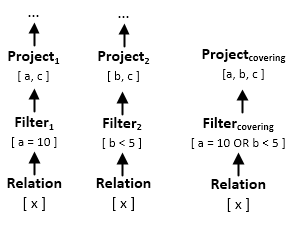
\includegraphics[scale=0.75]{figures/covering}
	\caption{Building covering subexpression example. The first and second trees are two SEs. The third tree is the CE}
   	\label{fig:covering}
\end{figure}